\documentclass[15pt,a4paper]{article}
\usepackage[portuguese]{babel}
\usepackage[utf8]{inputenc}
\usepackage{indentfirst}
\usepackage{graphicx}
\usepackage{verbatim}
\usepackage{float}
\usepackage{caption}
\usepackage{subcaption}
\begin{document}
\setlength{\textwidth}{16cm}
\setlength{\textheight}{22cm}

\title{\Huge\textbf{Implementação em Prolog do Jogo Oware}\linebreak\linebreak\linebreak
\Large\textbf{Relatório Final}\linebreak\linebreak

\includegraphics[height=6cm, width=7cm]{feup.pdf}\linebreak \linebreak
\Large{Mestrado Integrado em Engenharia Informática e Computação} \linebreak \linebreak
\Large{Programação em Lógica}\linebreak
}

\author{\textbf{Grupo 35:}\\ André Freitas - ei10036 \\ Rui Gonçalves - ei10100 \\\linebreak\linebreak \\
 \\ Faculdade de Engenharia da Universidade do Porto \\ Rua Roberto Frias, s\/n, 4200-465 Porto, Portugal \linebreak\linebreak\linebreak
\linebreak\linebreak\vspace{1cm}}
%\date{Junho de 2007}
\maketitle
\thispagestyle{empty}
\newpage
\section*{Resumo}
Este relatório tem o objetivo de descrever a implementação do Jogo Oware numa linguagem de programação lógica em matemática que é o Prolog. O jogo em questão é de tabuleiro, jogando-se com sementes, sendo muito popular na República do Gana. Apesar da simplicidade das regras tem um forte componente estratégico.\\
\indent O jogo  Oware foi implementado com recurso a listas para representar o tabuleiro e para representar as propriedades dos jogadores, estando organizando em módulos de manipulação do tabuleiro, rotinas de jogo, inteligência artificial, interfaces e predicados de teste. Existe ainda a possibilidade de jogar contra o computador com 2 níveis diferentes. Com isto, conseguiu-se uma interface de texto, não muito rica, mas adequada tendo em conta o contexto deste trabalho.


%*************************************************************************************************
%************************************************************************************************
\newpage
\renewcommand{\contentsname}{Índice}
\tableofcontents

%************************************************************************************************
%************************************************************************************************

\newpage
\section{Introdução}
Pretende-se explorar as capacidades do Prolog para representar um jogo e as suas regras através deste trabalho. Um jogo é uma excelente maneira de enriquecer o conhecimento na representação e estruturação dos dados bem como a aplicação de regras do jogo traduzidas nesta linguagem. \\
\indent A implementação em questão é em modo de texto, não sendo muito refinada no sentido da apresentação mas sim na componente das funcionalidades. \\
\indent Neste documento pretende-se apresentar a descrição do problema, a representação dos estados do jogo em estruturas conhecidas em Prolog, a representação das jogadas, a visualização do tabuleiro, a inteligência artificial e os aspetos de desenvolvimento do projeto.

\section{Descrição do Problema}
O Oware é dos jogos de tabuleiro mais antigos do mundo, tendo sido inventado há mais de 7 mil anos. É jogado por todo o Globo e não existem certezas relativamente à sua origem, porém, atribui-se a sua autoria tradicionalmente ao continente Africano. Atualmente é o jogo mais popular na República do Gana sendo um fenómeno nacional.

\begin{figure}[h!]
\begin{center}
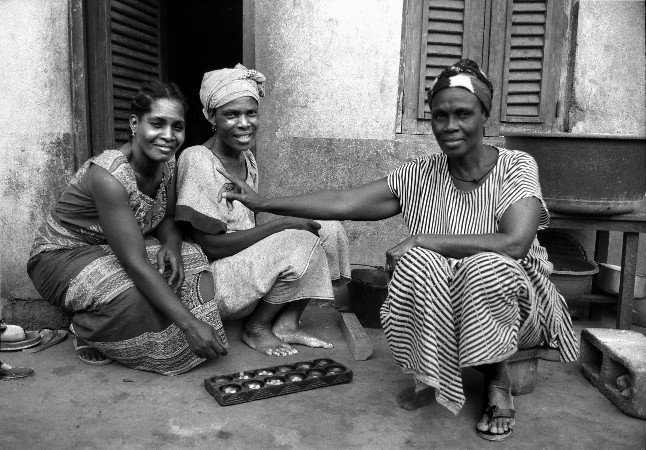
\includegraphics[scale=20]{awale.jpg}
\caption{Pessoas jogando tradicionalmente o Oware}
\label{fig:traditional}
\end{center}
\end{figure}

Como se pode constatar pela Figura 1, existe um tabuleiro com 2x6 cavidades onde se colocam sementes ou feijões. Existem muitas interpretações das regras deste jogo, pelo que iremos adotar apenas a que é mais conhecida. Assim, o jogo começa com 4 sementes em cada buraco. Os jogadores jogam alternadamente, e em cada jogada tira-se as sementes de um buraco da nossa linha de jogo e vai-se distribuindo as sementes no sentido anti-horário.
\begin{figure}[H]
\begin{center}
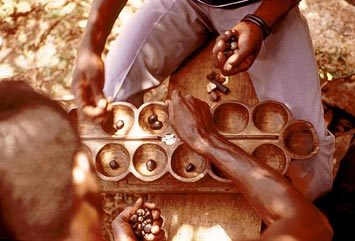
\includegraphics[scale=0.5]{oware.jpg}
\caption{Distribuição das sementes}
\label{fig:peoplePlaying}
\end{center}
\end{figure}
 \indent Quando distribuirmos a última semente e se colocarmos num buraco do adversário e esse sítio ficar com 2 ou 3 sementes, capturamos essas sementes. O jogo termina quando um jogador capturar 25 sementes ou ambos os dois jogadores capturarem 24 sementes (empate).

\subsection{Ilustração de jogadas}
Nas seguintes ilustrações serão descritas duas situações de jogos fundamentais. Pede-se especial atenção para as ilustrações, dado que é necessário estar atento às situações que descrevem para perceber o jogo.\\
\indent Nesta primeira situação o jogo está a começar e o jogador vai distribuir a segunda cavidade de sementes. Assim, as sementes ficaram distribuídas e não houve captura. De notar novamente que o sentido da distribuição das sementes é anti-horário e que o jogador só pode retirar as sementes da sua linha.
\begin{figure} [H]
        \centering
        \begin{subfigure}[f]{0.3\textwidth}
                \centering
                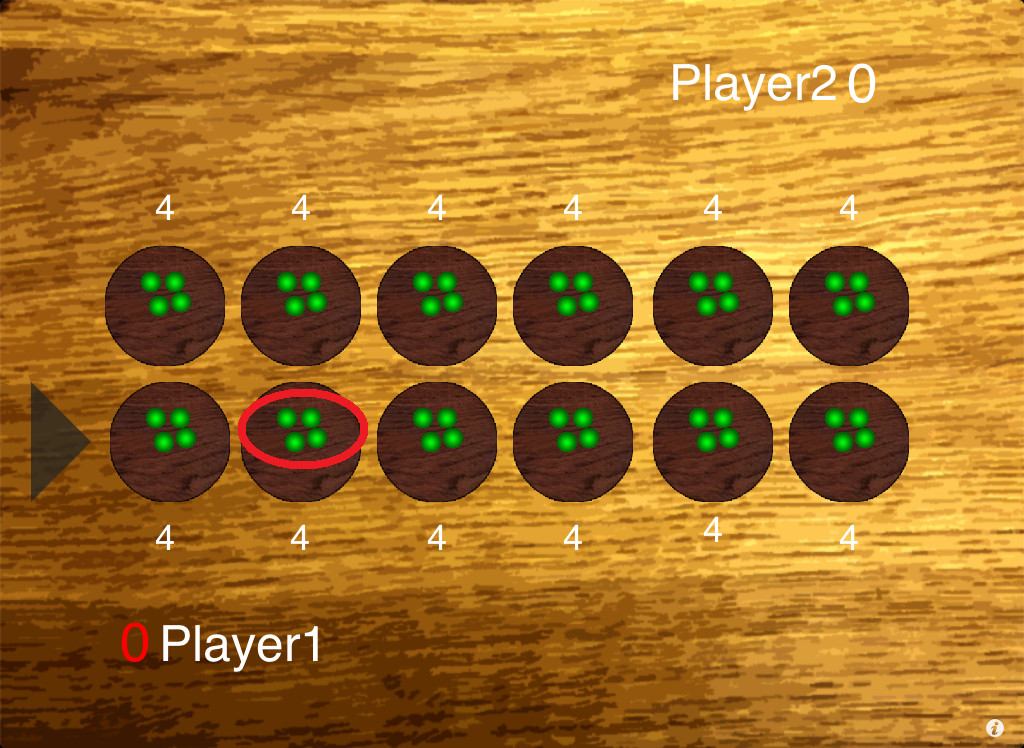
\includegraphics[scale=0.2]{iniciodoJogo.png}
				\caption{Estado Inicial do Jogo}
                \label{fig:inicioJogo}
        \end{subfigure}%
        \quad  \quad
        \begin{subfigure}[f]{0.3\textwidth}
                \centering
                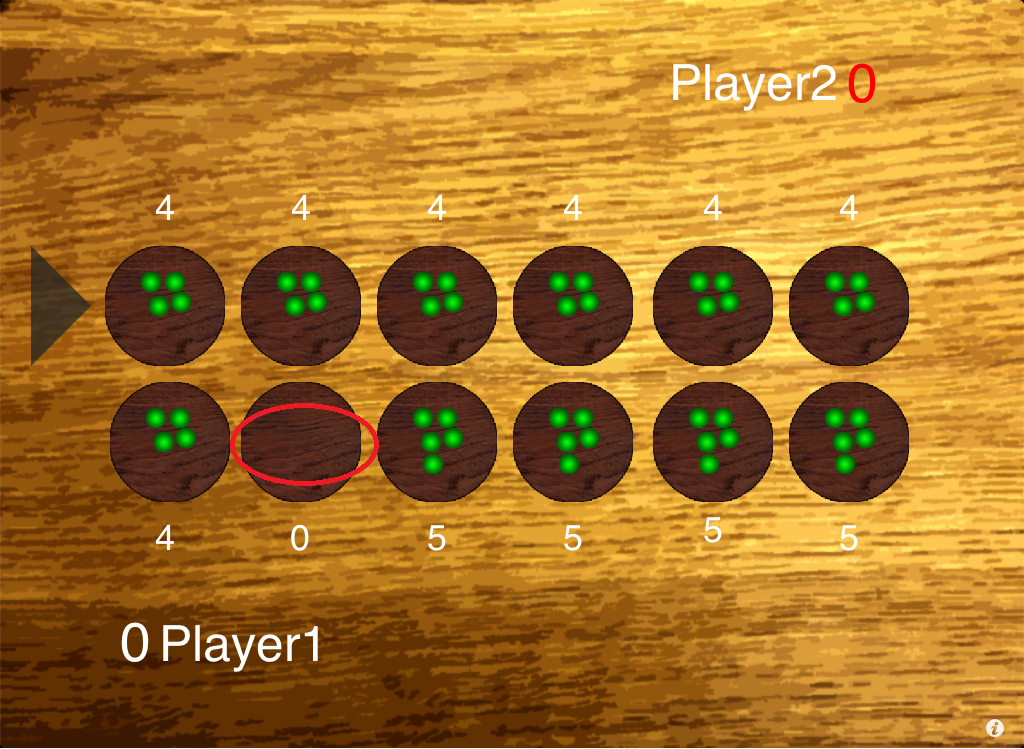
\includegraphics[scale=0.2]{semCaptura.png}
				\caption{Jogada sem Captura}
				\label{fig:semCaptura}
        \end{subfigure}
\end{figure}

A outra jogada importante é a da captura de sementes, ou seja, quando um jogador ao distribuir a última semente calha numa linha do seu adversário, ficam 2 ou 3 sementes nesse sítio, capturando-as. Atenção que se a meio da distribuição das sementes conseguir este número nas cavidades, não as pode capturar, por isso é só na semente final. Destaca-se esta situação dado que existem várias interpretações relativas a esta regra.

\begin{figure} [H]
        \centering
        \begin{subfigure}[f]{0.3\textwidth}
                \centering
                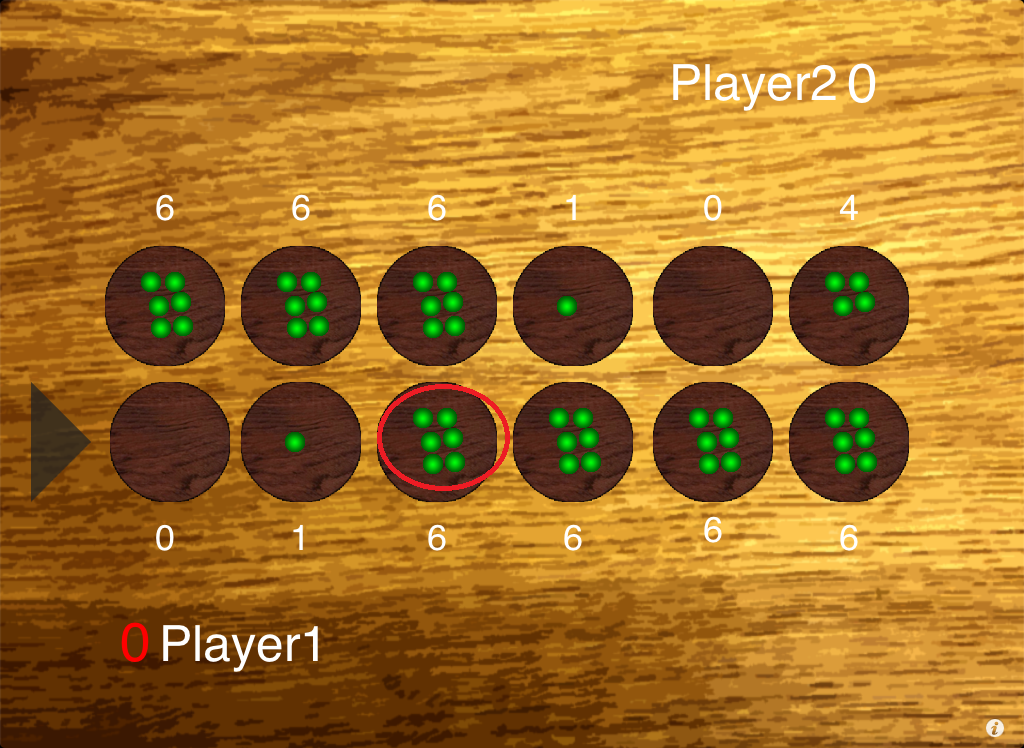
\includegraphics[scale=0.2]{antesCaptura.png}
				\caption{Antes da Captura}
                \label{fig:inicioJogo}
        \end{subfigure}%
        \quad  \quad
        \begin{subfigure}[f]{0.3\textwidth}
                \centering
                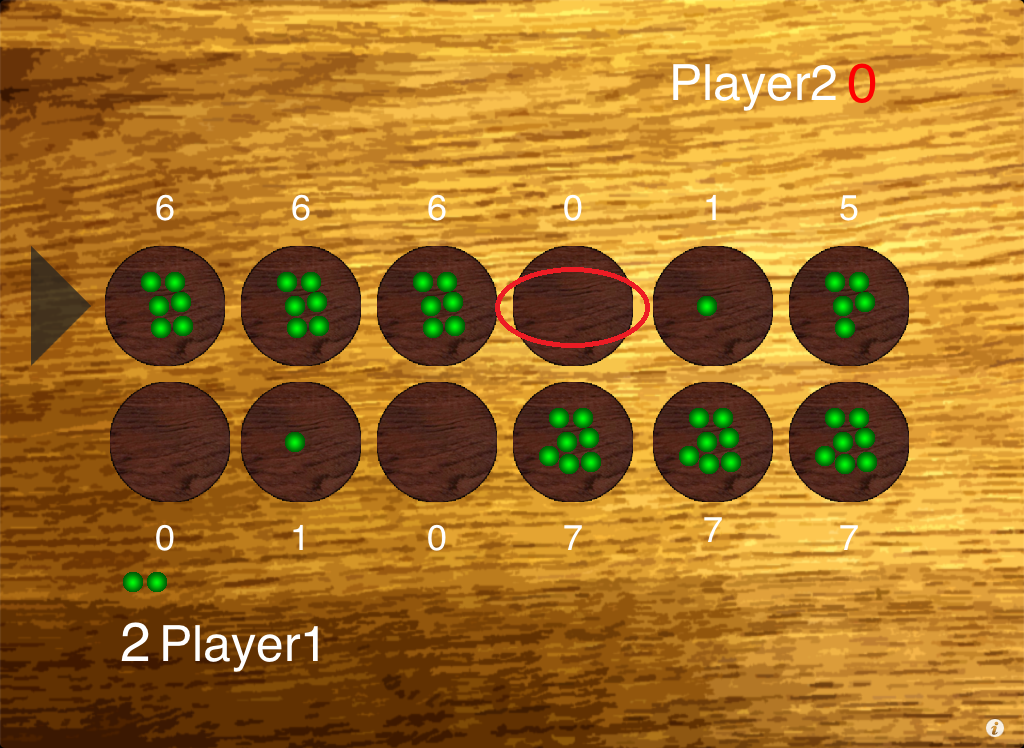
\includegraphics[scale=0.2]{captura.png}
				\caption{Após a Captura de Sementes}
				\label{fig:semCaptura}
        \end{subfigure}
\end{figure}

Pode-se constatar assim a simplicidade do jogo, mas apesar disso requer um componente estratégico para que se possa ganhar, tentando prever-se uma panóplia de jogadas possíveis para vencer o adversário e maximizar as nossas capturas.

\section{Arquitectura do Sistema}
Ora, como referido anteriormente, o sistema é decomposto em módulos o que permite um melhor isolamento no desenvolvimento e manutenção futura do código. Assim sendo, os módulos são os seguintes:
\begin{enumerate}
  \item oware.pl - possui todos os predicados inerentes à rotina de jogo;
  \item owareBoard.pl - contém os predicados para manipular e aceder à estrutura do tabuleiro;
  \item owareCLI.pl - alberga os predicados que interagem na consola de texto com o utilizador;
  \item owareAI.pl - módulo que contém os predicados para os bots;
  \item owareTest.pl - módulo que possui testes considerados pertinentes;
\end{enumerate}

\indent Destaca-se a atenção na análise do código dos predicados gameRoutine, aiPlay e playSeeds, que são o ponto de partida para a compreensão da implementação geral deste projecto.

\indent Para começar o jogo, basta fazer uma consulta ao ficheiro oware.pl e invocar o predicado startGame que recebe 2 parâmetros, que são os tipos do jogador 1 e 2, que podem ser human, bot1 ou bot2. Assim sendo, se pretende um jogo entre um humano e um bot de nível 2, será startGame(human,bot2), começando o primeiro jogador a jogar, visto que o turn é invocado com o valor 1 dentro do predicado startGame. 


\newpage

\subsection{Protocolo de mensagens com o visualizador}
Para a implementação com o visualizador 3D, será criado um módulo que terá o nome "owareServer.pl", usando a comunicação por socket do Sicstus com o seguinte protocolo de mensagens:
\begin{verbatim}
     +----------------+                            +----------------+
     |   LAIG APP     |   beginGame human bot2     |  Oware Server  |
     |----------------|+-------------------------->|----------------|
     |                |                      ack   |                |
     |                |<--------------------------+|                |
     |                |                            |                |
     |                |                            |                |
     |                |              playerTurn 1  |                |
     |                |<--------------------------+|                |
     |                |  gameStatus (board) 1 2    |                |
     |      C++       |<--------------------------+|     Prolog     |
     |                |  playerChooses 1           |                |
     |                |+-------------------------->|                |
     |                |                            |                |
     |                |                            |                |
     |                |                            |                |
     |                |      endGame victory 1     |                |
     |                |<--------------------------+|                |
     +----------------+                            +----------------+
\end{verbatim}
Assim sendo, a sintaxe das mensagens, é a seguinte:
\begin{enumerate}
\item beginGame (player1Type) (player2Type) - indica a informação para iniciar o jogo;
\item ack - confirma o início do jogo;
\item playerTurn (1 or 2) - indica qual é o jogador que vai jogar;
\item gameStatus (board) (player1 score) (player2 score) - indica o estado do jogo;
\item playerChoose (1-6) - indica qual a posição escolhida pelo jogador;
\item endGame (victory (1 or 2)) or (draw) - sinaliza o fim do jogo.
\end{enumerate}

Dado que as mensagens que são passadas entre os sistema são relativamente simples, este formato é suficiente, porém, se se tratasse de um sistema que necessitasse de algo mais complexo, faria todo o sentido usar um formato para representar estruturas de dados como JSON, pois do lado da aplicação de LAIG em C++ existem bibliotecas para tal.

\section{Módulo de Lógica do Jogo}
Como descrito anteriormente, o projecto foi implementado em módulos para as diferentes camadas do jogo Oware. Nesta secção serão apresentada as soluções que desenvolvemos relativa sa cada componente lógica do jogo.

\subsection{Representação do Estado do Jogo}
Ora, todos os jogos possuem o ciclo, sendo o jogo representado em cada iteração por estruturas conhecidas. Assim, existe a lista que representa o tabuleiro e cada jogador tem uma lista que possui o tipo de jogador(human, bot1,bot2) e a sua pontuação. Um exemplo possível de um estado de jogo é o seguinte:
\begin{verbatim}
gameRoutine([[1,0,7,0,0,0],[0,4,2,1,1,0]],[human,20],[bot1,12],1).
\end{verbatim}

\subsection{Visualização do Estado do Jogo}
Ora o estado do jogo é visualizado pelo utilizador em modo de texto ou pelo visualizador CGI. O estado do jogo é apresentado pelo predicado:
\begin{verbatim}
 printBoard(Board,Player1Score,Player2Score).
\end{verbatim}


\subsection{Manipulação das Sementes do Tabuleiro}
O "core" deste projecto na abstracção do acesso ao tabuleiro, foi a implementação de processos inteligentes para aceder ao mesmo. Existem então duas maneiras de aceder às sementes. A primeira é pela indicação do número do jogador e o índice de 0 a 5 que corresponde à posição da sua linha no tabuleiro. A segunda forma e a que tornou o processo de distribuição de sementes extremamente fácil é o acesso pelo índice circular, implementando um acesso circular às listas. Assim, as posições circulares no tabuleiro são:
\begin{verbatim}
[5,4,3,2,1,0]
[6,7,8,9,10,11]
\end{verbatim}
Assim, se queremos aceder à posição 12, salta para a posição 0, o que é uma estratégia acertada para simplificar a manipulação do tabuleiro. Para uma compreensão mais aprofundada, recomenda-se a análise do código no ficheiro owareBoard.pl na secção "Board Predicates and Iterators". 

\subsection{Validação de Jogadas}
É necessário validar o input das posições quando se trata de um jogador Humano, pelo que simplesmente garante-se que é fornecida uma posição de 1 a 6. O predicado readUserInput pode ser encontrado no ficheiro owareCLI.pl.
\begin{verbatim}
readUserInput(Pos):-
	(read(Pos),Pos >0,Pos <7);
	write(':( Invalid Position!. Insert again:'),
	readUserInput(Pos).
\end{verbatim}

\subsection{Execução de Jogadas}
Ora o predicado mais importante é claramente o da execução de jogadas, sendo o playSeeds que recebe 5 parâmetros que são o tabuleiro, número do jogador, índice de 0 a 5, novo tabuleiro e pontuação da jogada. O índice começa em 0 e não em 1 por ser mais ortodoxo no acesso às listas. De notar que o jogador 1 joga na primeira lista e o 2 na segunda lista. Um exemplo de uma chamada poderia ser:
\begin{verbatim}
playSeeds([[1,0,7,0,0,0],[0,4,2,1,1,0]],1,2,[[2,1,0,0,0,0],[1,5,0,0,0,0]],7).
\end{verbatim}

\subsection{Jogadas Válidas}
Ora, o jogador pode jogar todas as posições da sua linha do tabuleiro, exceptuando quando a posição escolhida não ter sementes. Se tal acontecer, dado que existe um predicado para obter as sementes de uma posição, o programa simplesmente pede de novo uma posição ao jogador. Assim sendo, não se torna útil neste tipo de jogo de tabuleiro, com uma restrição muito simples, criar um predicado que a partir de um tabuleiro devolva as jogadas válidas. Acresce ainda o facto de que, se na linha do tabuleiro do jogador em questão, todas as posições não tiverem sementes, o jogo cede a vez ao próximo jogador até que existe pelo menos 1 semente para jogar. 


\subsection{Final do Jogo}
O jogo acaba quando um dos jogadores chegar aos 25 pontos ou ambos os jogadores empatarem por 24 pontos. Esta restrição é garantida no predicado gameRoutine, sendo o código correspondente a estas situações o seguinte:
\begin{verbatim}
gameRoutine(_,Player1,Player2,_):-
	Player1=[_,P1Score],
	Player2=[_,P2Score],
	P1Score=24,P1Score=P2Score,
	write('You Both Win!').

gameRoutine(_,Player1,Player2,_):-
	Player1=[_,P1Score],
	Player2=[_,P2Score],
	(
		(P1Score>=25),
		write('\nPlayer 1 Wins!');

		(P2Score>=25),
		write('\nPlayer 2 Wins!')
	).
\end{verbatim}

\subsection{Cálculo da Jogada do Computador}
Os bots têm 2 níveis de dificuldade, sendo o bot1 um jogador que escolhe posições aleatoriamente e o bot2 um jogador com capacidade de decidir qual a jogada que lhe irá dar mais pontos, aplicando uma estratégia gananciosa (greedy algorithms). Foi colocado um sleep de um segundo quando o bot joga para que o utilizador possa aperceber-se da sua presença facilmente.\\
\indent De notar que o jogo em si, poderá levar um tempo considerável a acabar, dado que chega-se a um ponto em que ambos os jogadores impedem o adversário de pontuar, ou seja, esta nuance também se reflecte nos bots que, ao jogararem entre si, podem levar imenso tempo a finalizar o jogo.\\
\indent A invocação do bot é feita pelo aiPlay que tem como parâmetros o número do jogador, o tabuleiro, a posição e o tipo de bot (bot1 ou bot2).

\begin{verbatim}
aiPlay(PlayerNum,Board,Pos,BotType):-
	% If it's level 1 bot
	BotType = bot1,
	stupidBot(PlayerNum,Board,Pos);

	% If it's level 2 bot and score
	BotType = bot2,
	(
		aiTryAll(Board, PlayerNum, ScoreList,0),
		scoreListGetPos(ScoreList,1,Pos,MaxScore),
		MaxScore>0
	);
	%write('Going random...\n'),
	aiPlay(PlayerNum,Board,Pos,bot1).

\end{verbatim}


\subsection{Mensagens com o visualizador}
A integração da troca de mensagems com o utilizador será feita na secção onde se imprime o tabuleiro e onde se obtem a posição das sementes por parte do jogador. No nível mais alto da implementação será o predicado readCGIUserInput(Pos), que irá recorrer ao predicados de troca de mensagen: sendMessage(Message) e readMessage(Message). Estas funcionalidades serão implementadas em conjunto com o terceiro prático de LAIG, pelo será esse o momento oportuno para o seu desenvolvimento.


\section{Interface com o Utilizador}
A interface com o utilizador é relativamente simples, usando-se a linha de comandos do interpretador Prolog. \\
\indent A cada iteração do jogo o tabuleiro é apresentado, pedindo-se ao utilizador que escreve a posição que quer jogar, ou se se tratar do bot, imprime-se a sua escolha. Para começar o jogo basta invocar o predicado startGame/2.

\begin{figure}[h!]
	\begin{center}
	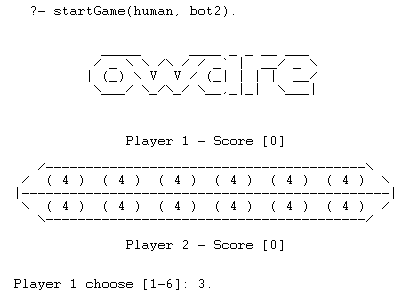
\includegraphics[scale=1]{owareBeginGame.png}
	\caption{Início do Jogo}
	\label{fig:Comeco}
	\end{center}
\end{figure}


\begin{figure}[h!]
	\begin{center}
	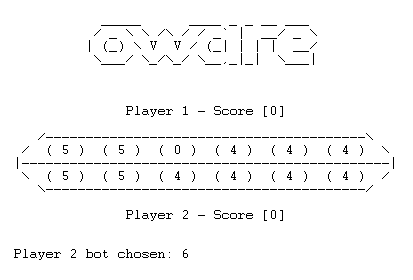
\includegraphics[scale=1]{owareBotPlays.png}
	\caption{Um bot jogou}
	\label{fig:Comeco}
	\end{center}
\end{figure}

\begin{figure}[h!]
	\begin{center}
	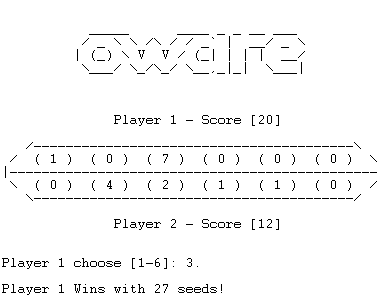
\includegraphics[scale=1]{owareVictory.png}
	\caption{Vitória de um Jogador}
	\label{fig:Comeco}
	\end{center}
\end{figure}
\newpage
\section{Conclusões e Perspetivas de Desenvolvimento}
Para um programador comum que está habituado a linguagens funcionais, no primeiro contato com o Prolog é normal sentir-se um bocado limitado devido ao paradigma que está habituado a ter no desenvolvimento de soluções. Porém, após um período, consegue aperceber-se da potencialidade que esta linguagem tem, especialmente em computar soluções. \\
\indent O desenvolvimento do Oware em Prolog teve um ritmo estável, apesar de que se teve obviamente momentos em que foram alocados períodos de tempos consideráveis para despitar bugs que numa linguagem funcional seriam triviais. Apesar disso, cumpriram-se os objetivos inicialmente propostos, o que se traduz num desafio superado com sucesso.
\\ \indent Ora reforça-se que esta implementação se enquadra no contexto da Unidade Curricular de programação em lógica e admite-se que com o Prolog consegue-se mais facilmente computar soluções, que envolvam processos heurísticos e recursivos. Porém, existe uma perda enorme na legibilidade do código visto que as instruções que habitualmente descrevem um corpo de uma função, são substituídas por uma série de predicados, sendo necessário interpretar todos os parâmetros que esses predicados contêm, tornando mais difícil a compreensão das decisões tomadas. 
\\ \indent Os interpretadores SWI Prolog e Sicstus, foram usadas para correr o nosso código, porém, carecem de um bom editor de texto, pelo que a melhor solução encontrada foi o Sublime Text 2 que possui a sintaxe de Prolog, tornando o desenvolvimento muito mais produtivo. Outro problema encontrado é que estes em certos aspectos, não são uniformes entre si relativamente ao Standard do Prolog. Possivelmente estes problemas serão concerteza resolvidos no futuro com a motivação da comunidade que desenvolve em Prolog.
\\ 
\indent Consideramos que fizemos uma implementação eficiente do Oware e, dado que o nosso esquema de tabuleiro é simples, foi fácil representá-lo em modo de texto, pois para um jogo mais complexo seria concerteza uma barreira a ultrapassar. O desenvolvimento de testes nos aspectos críticos do Jogo garantem que entregamos um produto final. Pode-se sugerir no futuro uma abordagem de testes mais exaustiva mas para projectos que tenham um grau de complexidade superior. 



\newpage
\section{Bibliografia}
\begin{thebibliography}{9}

\bibitem{oware}
  The Oware Society.
  2010.
  \emph{ Oware- Played all over the World}.
  Acedido a 4 de Outubro de 2012.
  http://www.oware.org.
  
  \bibitem{Figura 1}
  Awale.jpg.
  2006.
  \emph{A game of awale}.
  Acedido a 4 de Outubro de 2012.
  http://upload.wikimedia.org/wikipedia/commons/1/14/Awale.jpg.
  
   \bibitem{Figura 2}
	oware.jpg.
  \emph{Playing Oware in Ghana}.
  Acedido a 4 de Outubro de 2012.
  http://exploringafrica.matrix.msu.edu/teachers/events/oware.jpg.
  
   \bibitem{Figura 3}
	Easy Oware
	2012.
  \emph{Play the classic strategy game from Africa}.
  Acedido a 2 de Outubro de 2012.
  http://itunes.apple.com/br/app/easy-oware/id408219960?mt=8.
  
  \bibitem{Prolog Random}
  SICStus Prolog.
  \emph{SICStus Prolog - Random Number Generator}.
    Acedido a 1 de Novembro de 2012.
  http://www.sics.se/sicstus/docs/3.7.1/html/sicstus\textunderscore23.html.

\end{thebibliography}

\newpage
\appendix
\section{Código Implementado}
Módulo oware.pl
 \begin{verbatim}
 % Include modules
:- consult(owareCLI).
:- consult(owareBoard).
:- consult(owareAI).
:-use_module(library(system)).
	
% updateScoreandTurn/7
% Updates the user score and the player turn
% Args: Current Turn, Score done, Player 1 Score, Player 2 Score, New Turn, New Player 1 Score, New Player 2 Score
updateScoreandTurn(Turn, Score, P1Score, P2Score, TurnNew, P1ScoreNew, P2ScoreNew):-
	((Turn =1,
	P1ScoreNew is P1Score + Score,
	P2ScoreNew=P2Score);

	(Turn=2,
	P2ScoreNew is P2Score + Score,
	P1ScoreNew=P1Score)),
	TurnNew is Turn mod 2 +1.

% Give the player that plays now
whoPlaysNow(Turn,Player1,Player2,PlaysNow):-
	Turn=1,PlaysNow=Player1;
	Turn=2,PlaysNow=Player2.

% GameRoutine/5
% Here is where the magic goes 
% Args: Board, Player 1 Score, Player 2 Score, Turn , BotType
gameRoutine(_,Player1,Player2,_):-
	Player1=[_,P1Score],
	Player2=[_,P2Score],
	P1Score=24,P1Score=P2Score,
	write('You Both Win!').

gameRoutine(_,Player1,Player2,_):-
	Player1=[_,P1Score],
	Player2=[_,P2Score],
	(
		(P1Score>=25),
		write('\nPlayer 1 Wins with '), write(P1Score), write(' seeds!');

		(P2Score>=25),
		write('\nPlayer 2 Wins with '), write(P2Score), write(' seeds!')
	).

gameRoutine([H|[Th|Tt]],Player1,Player2,Turn):-
	( 
		(Turn=1,H=[0,0,0,0,0,0],\+(Th=[0,0,0,0,0,0]));
		(Turn=2,Th=[0,0,0,0,0,0],\+(H=[0,0,0,0,0,0]))
	),
	TurnNew is Turn mod 2 +1,
	write('\nYou have no seeds to play :( passing turn...\n'),
	sleep(1),
	gameRoutine([H|[Th|Tt]],Player1,Player2,TurnNew).

gameRoutine(Board,Player1,Player2,Turn):-
	Player1=[P1Type,P1Score],
	Player2=[P2Type,P2Score],
	printBoard(Board,P1Score,P2Score),

	% User plays
	isBotThisTurn(Turn,Player1,Player2,IsBot),
	whoPlaysNow(Turn,Player1,Player2,PlaysNow),
	PlaysNow=[PlayerType,_],
	write('Player '),write(Turn),
	(
		IsBot=true,
		aiPlay(Turn,Board,Pos,PlayerType),
		write(' bot chosen: '), write(Pos), nl,sleep(1);
		% else
		write(' choose [1-6]: '),
		readUserInput(Pos)
	),

	% Call the game routine again
	(
		% If player played positon with seeds
		(playSeeds(Board,Turn,Pos - 1,NewBoard,Score),
	 	\+(NewBoard=Board) ,
		updateScoreandTurn(Turn,Score,P1Score,P2Score,TurnNew,P1ScoreNew,P2ScoreNew),
		Player1New=[P1Type,P1ScoreNew],
		Player2New=[P2Type,P2ScoreNew],
		gameRoutine(NewBoard,Player1New,Player2New,TurnNew))
		
		; % else
		gameRoutine(Board,Player1,Player2,Turn)
	).
	
% StartGame/0
% Call this predicate to start playing the game
startGame(Player1Type,Player2Type):- initBoard(B),gameRoutine(B,[Player1Type,0],[Player2Type,0],1). 
\end{verbatim}
Módulo owareBoard.pl
\begin{verbatim}
% ****************************************************************
%                           Lists predicates
% ****************************************************************

% replace/4
% Replaces an element in a list
% Args: List, Position, NewValue, NewList
replace([_|T],0,X,[X|T]).
replace([H|T],N,X,[H|T2]):- 
	N>0, 
	N1 is N-1,
	replace(T,N1,X,T2).
	
% element/3
% Get an element of a list
% Args: List, Position, Value
element([H|_],0,H).
element([_|T],N,Val):-
	N>0,
	N2 is N-1,
	element(T,N2,Val).
	
% elementPlus/4
% Adds an integer to an element in a list
% Args: List, Position, Value, NewList
elementPlus(List,I,Value,NewList):-
	element(List,I,Oldval),
	Newval is Oldval+Value,
	replace(List,I,Newval,NewList).
	
% elementMinus/4
% Subtract and integer from an element in a list
% Args: List, Position, Value, NewList
elementMinus(List,I,Value,NewList):-
	element(List,I,Oldval),
	Newval is Oldval-Value,
	replace(List,I,Newval,NewList).

% ****************************************************************
%                  Board Predicates and Iterators
% ****************************************************************

% initBoard/1
% Starts the board with the default seeds
% Args: Board
initBoard([[4,4,4,4,4,4],[4,4,4,4,4,4]]).

% addSeeds/5
% Adds seeds into the Board
% Args: Player Number, Board, Index [0-6], Seeds, New Board
addSeeds(PlayerNum,[H|[Th|Tt]],I,Seeds,[Hnew|Tnew]):-
	PlayerNum=1,
	elementPlus(H,I,Seeds,Hnew),
	Tnew = [Th|Tt];
	PlayerNum=2,
	elementPlus(Th,I,Seeds,T2),
	Tnew = [T2|[]],
	Hnew = H.	

% removeSeeds/5
% Remove seeds in the board
% Args: Player Number, Board, Index [0-5], Seeds, New Board
removeSeeds(PlayerNum,[H|[Th|Tt]],I,Seeds,[Hnew|Tnew]):-
	PlayerNum=1,
	elementMinus(H,I,Seeds,Hnew),
	Tnew = [Th|Tt];
	PlayerNum=2,
	elementMinus(Th,I,Seeds,T2),
	Tnew = [T2|[]],
	Hnew = H.
		
% getSeeds/4
% Returns the number of seeds of the board
% Args: Player Number, Board, Index [0-5], Seeds, New Board
getSeeds(PlayerNum,[H|[Th|_]],I,Seeds):-
	PlayerNum=1,
	element(H,I,Seeds);
	PlayerNum=2,
	element(Th,I,Seeds).
	
% Circular Acces to the Board
% The way to access it is the following (CCW :D ).
% [ 5 4 3 2 1 0 ]
% [ 6 7 8 9 10 11 ]

% getCircularIndex/3
% Converts the player,index to circularIndex
% Args: Player Number, Index[0-5], Circular Index
getCircularIndex(PlayerNum,I,CircularIndex):-
		PlayerNum =1,
		CircularIndex is 5-I;
		PlayerNum=2,
		CircularIndex is 6+I.

% getBoardIndex/3
% Converts the given circular index to player linear index. 
% This predicate is necessary because the access to the board
% is continuous in counter clock wise.
% Args: Circular Index, Player Number, Line Index[0-5]
getBoardIndex(CircularIndex, PlayerNum, LineIndex):-
	CircularIndex > 11,
	Index is CircularIndex mod 11 - 1,
	getBoardIndex(Index,PlayerNum,LineIndex);
	CircularIndex > 5,
	CircularIndex < 12,
	LineIndex is CircularIndex-6,
	PlayerNum=2;
	CircularIndex>=0,
	CircularIndex<6,
	LineIndex is 5-CircularIndex,
	PlayerNum=1.

% getSeedsCircular/3
% Get the Seeds by the circular index
% Args: Board, CircularIndex, Seeds
getSeedsCircular(Board,CircularIndex,Seeds):-
	getBoardIndex(CircularIndex, PlayerNum, LineIndex),
	getSeeds(PlayerNum,Board,LineIndex,Seeds).
	
% addSeedsCircular/4
% Add seeds to a position of the board
% Args: Board, CircularIndex, Seeds, NewBoard
addSeedsCircular(Board,CircularIndex,Seeds,NewBoard):-
	getBoardIndex(CircularIndex, PlayerNum, LineIndex),
	addSeeds(PlayerNum,Board,LineIndex,Seeds,NewBoard).

% removeSeedsCircular/4
% Removes the Seeds in the given circular position
% Args: Board, CircularIndex, Seeds, NewBoard
removeSeedsCircular(Board,CircularIndex,Seeds,NewBoard):-
	getBoardIndex(CircularIndex, PlayerNum, LineIndex),
	removeSeeds(PlayerNum,Board,LineIndex,Seeds,NewBoard).

	% placeSeeds/5
% Distribute the seeds from a given position
% Args: Board, Circular Index, Seeds, NewBoard, Final Circular Index
placeSeeds(TempBoard,CircularIndex,1,NewBoard,FinalIndex):-
	addSeedsCircular(TempBoard,CircularIndex,1,NewBoard),
	FinalIndex is CircularIndex.	

placeSeeds(TempBoard,CircularIndex,Seeds,NewBoard,FinalIndex):-
	addSeedsCircular(TempBoard,CircularIndex,1,TempBoard1),
	CircularIndex2 is CircularIndex + 1,
	NSeeds is Seeds - 1,
	placeSeeds(TempBoard1,CircularIndex2,NSeeds,NewBoard,FinalIndex).

% playSeeds/5
% Play the seeds from a given position
% Args: Board, Player Number, Index, NewBoard, Score
playSeeds(Board,PlayerNum,I,Board,0):-
	getCircularIndex(PlayerNum,I,CircularIndex),
	getSeedsCircular(Board,CircularIndex,0). % Case when there are 0 seeds

playSeeds(Board,PlayerNum,I,NewBoard,Score):-
	getCircularIndex(PlayerNum,I,CircularIndex),
	getSeedsCircular(Board,CircularIndex,Seeds),
	removeSeedsCircular(Board,CircularIndex,Seeds,TempBoard),
	placeSeeds(TempBoard,CircularIndex+1,Seeds,TempBoard2,FinalIndex),
	captureSeeds(TempBoard2,PlayerNum,FinalIndex,NewBoard,Score).

% captureSeeds/5
% By giving the last position, the predicate capture the seeds in the oposite 
% way and compute the score.
% Args: Board, PlayerNum, Last Circular Index, NewBoard, Score
captureSeeds(Board,PlayerNum,IndexC,Board,0):-

	PlayerNum = 2,
	IndexC = -1 ; 
	PlayerNum = 2,
	IndexC >= 6 ,
	IndexC =< 11;
	
	PlayerNum = 1,
	IndexC >= 0,
	IndexC =< 5;
	
	getSeedsCircular(Board,IndexC,Seeds),
	Seeds > 3;
	
	getSeedsCircular(Board,IndexC,Seeds),
	Seeds < 2.
	
captureSeeds(Board,PlayerNum,IndexC,NewBoard,Score):-
	getSeedsCircular(Board,IndexC,Seeds),
	removeSeedsCircular(Board,IndexC,Seeds,TmpBoard),	
	NewIndexC is IndexC - 1,
	captureSeeds(TmpBoard,PlayerNum,NewIndexC,NewBoard,TmpScore),
	Score is TmpScore + Seeds.
	
\end{verbatim}

Módulo owareAI.pl
\begin{verbatim}
% Include modules
:- consult(owareBoard).
:- use_module(library(random)).

% aiPlay/4
% The Computer Plays trying to have the best score at each stage
% Args: Player Number, Board, Position[1-6]
aiPlay(PlayerNum,Board,Pos,BotType):-
	% If it's level 1 bot
	BotType = bot1,
	stupidBot(PlayerNum,Board,Pos);

	% If it's level 2 bot and score
	BotType = bot2,
	(
		aiTryAll(Board, PlayerNum, ScoreList,0),
		scoreListGetPos(ScoreList,1,Pos,MaxScore),
		MaxScore>0
	);
	%write('Going random...\n'),
	aiPlay(PlayerNum,Board,Pos,bot1).

	

% aiTryAll/4
% Try all the possible positions and put the scores in the list
%Args: Board, Player Number, Score List, Index that starts with 0 N[0-5]
aiTryAll(Board, PlayerNum,[Score],5):-
	playSeeds(Board,PlayerNum,5,_,Score).

aiTryAll(Board, PlayerNum, ScoreList,N):-
	N<5,
	playSeeds(Board,PlayerNum,N,_,Score),
	%write('N: '), write(N),write(' - Score: '), write(Score),nl,
	NewN is N+1,
	aiTryAll(Board,PlayerNum,NewScoreList,NewN),
	append([Score],NewScoreList,ScoreList).

% scoreListGetPos/4
% Gets the position of the maximum score
% Args: Score List, Max Score Position[1-6], Max Score
scoreListGetPos(ScoreList,6,MaxScorePos,MaxScore):-
	ScoreList=[Score|_],
	MaxScore=Score,
	MaxScorePos=6.

scoreListGetPos(ScoreList,N,MaxScorePos,MaxScore):-
	ScoreList=[Score|T],
	NewN is N+1,
	scoreListGetPos(T,NewN,MaxScorePosNext,MaxScoreNext),
	(
		Score > MaxScoreNext,
			MaxScorePos=N,
			MaxScore=Score;
		% else
			MaxScorePos=MaxScorePosNext,
			MaxScore=MaxScoreNext
	).

% isBotThisTurn/4
% Check if at this turn is a bot
% Args: Turn, Player 1, Player 2, Bool value
isBotThisTurn(Turn,Player1,Player2,Bool):-
	Player1=[P1Type,_],
	Player2=[P2Type,_],
	(
		Turn=1,
		(
			(P1Type=bot1; P1Type=bot2),
			Bool=true;
			Bool=false
		);
		Turn=2,
		(
			(P2Type=bot1; P2Type=bot2),
			Bool=true;
			Bool=false
		)
	).

% choosePositionWithSeeds/3
% Choose a position that have Seeds 
choosePositionWithSeeds(_,Board,Pos):-
	Board=[H|[Th|_]],
	(
		(H=[0,0,0,0,0,0]; Th=[0,0,0,0,0,0]),
		Pos = -1
	).

choosePositionWithSeeds(PlayerNum,Board,Pos):-
	%write('Eu estou aqui'),
	Board=[H|[Th|_]],
	(
		PlayerNum=1,
		findNonZeroElement(H,0,Index);

		PlayerNum=2,
		findNonZeroElement(Th,0,Index)
	),
	Pos is Index+1.
	
% findNonZeroElement/2
% Finds an element that is greater than zero
findNonZeroElement([],_,-1).
findNonZeroElement([H|T],N,Index):-
	H>0, Index=N;
	% Else
	NewN is N+1,
	findNonZeroElement(T,NewN,Index).

%stupidBot/3
%dah it's a stupid bot! it just picks a random from 1 to 6
stupidBot(PlayerNum,Board,Pos):-	
	random(1,7,Pos),
	Index is Pos - 1,
	getSeeds(PlayerNum,Board,Index,Seeds),
	Seeds >0;
	% seeds are >0 or calls again
	stupidBot(PlayerNum,Board,Pos).
\end{verbatim}

Módulo owareCLI.pl

\begin{verbatim}
% printBoardLine/1
% Prints a line of the board
% Args: list
printBoardLine([]).
printBoardLine([H|T]):-
	write(' ( '),
	write(H),
	write(' ) '),
	printBoardLine(T).
	
% printLogo/0
% prints the game logo.
printLogo:-
	write('\n\n'),
	write('           _____      ____ _ _ __ ___\n'), 
	write('          / _ \\ \\ /\\ / / _` |  __/ _ \\ \n'),
	write('         | (_) \\ V  V / (_| | | |  __/ \n'),
	write('          \\___/ \\_/\\_/ \\__,_|_|  \\___| \n\n\n').

% printBoard/3
% prints the game board on screen and the players score.
% Args: Board, Player 1 Score, Player2 Score
printBoard([H|[Th|_]],P1Score,P2Score):-
	printLogo,
	write('\n'),
	write('              Player 1 - Score ['),
	write(P1Score),
	write(']\n\n'),
	write('   /----------------------------------------\\ \n'),
	write(' / '), printBoardLine(H),write(' \\ \n'),
	write('|----------------------------------------------|'),
	write('\n \\ '), printBoardLine(Th), write(' / \n'),
	write('   \\----------------------------------------/\n\n'),
	write('              Player 2 - Score ['),
	write(P2Score),
	write(']\n\n\n').
	
% Read user input
% Args: position [1-6]
readUserInput(Pos):-
	(read(Pos),Pos >0,Pos <7);

	write(':( Invalid Position!. Insert again:'),
	readUserInput(Pos).
\end{verbatim}

Módulo owareTest.pl

\begin{verbatim}
:- consult(oware).

% Test victory of Player 1 and Player 2
% Instructions: write position 3.
testVictoryPlayer1:- B=[[1,0,7,0,0,0],[0,4,2,1,1,0]],gameRoutine(B,[human,20],[human,12],1). 
testVictoryPlayer2:- B=[[0,4,2,1,1,0],[1,0,7,0,0,0]],gameRoutine(B,[human,12],[human,20],2). 

% Test when a player can't play because the row is [0,0,0,0,0,0]
% Instructions: write position 1 -> write position 1
testPlayer1CantPlay:- B=[[4,0,0,0,0,0],[0,0,0,4,5,3]],gameRoutine(B,[human,20],[human,12],1).
testPlayer2CantPlay:- B=[[0,0,0,4,5,3],[4,0,0,0,0,0]],gameRoutine(B,[human,12],[human,20],2).

% Test smart bot
% Instructions: the position should be allways 6 because it the one that have more score
testBotIsSmart1(Pos):- aiPlay(1,[[0,2,0,0,0,7],[1,2,3,4,5,6]],Pos,bot2).
% Instructions: the position should be allways 2 because it the one that have more score
testBotIsSmart2(Pos):- aiPlay(2,[[1,1,1,1,1,1],[0,7,0,0,2,0]],Pos,bot2).
% Instructions: you should expect 5
testBotIsSmartButCantScore(Pos):-aiPlay(1,[[0,0,0,0,1,2],[0,1,2,3,4,5]],Pos,bot2).

% Test dumb bot
% Instructions: the positions should be 2 or 6 because it can't compute the max score
testBotIsDumb1(Pos):- aiPlay(1,[[0,2,0,0,0,7],[1,2,3,4,5,6]],Pos,bot1).
\end{verbatim}
\end{document}
